
\vspace*{0.1in}
\begin{Large}
\textbf{SISTEMA DE CONTROL DE VERSIONES} \\
\end{Large}

\vspace*{0.1in}
\begin{large}
 El control de versiones es un sistema que registra los cambios realizados sobre un archivo o conjunto de archivos a lo largo del tiempo, de modo que puedas recuperar versiones específicas más adelante. Te permite revertir archivos a un estado anterior, revertir el proyecto entero a un estado anterior, comparar cambios a lo largo del tiempo.\\
\end{large}

\section{GitHub} 
GitHub es una forja (plataforma de desarrollo colaborativo) para alojar proyectos utilizando el sistema de control de versiones Git. Se utiliza principalmente para la creación de código fuente de programas de computadora. El software que opera GitHub fue escrito en Ruby on Rails. Desde enero de 2010, GitHub opera bajo el nombre de GitHub, Inc. Anteriormente era conocida como Logical Awesome LLC. El código de los proyectos alojados en GitHub se almacena típicamente de forma pública, aunque utilizando una cuenta de pago, también permite hospedar repositorios privados.

El 4 de junio de 2018, Microsoft compró GitHub por la cantidad de 7.500 millones de dólares.

\begin{itemize}
	\item SELECT last\_name, job\_id, salary AS Sal FROM employees;
	\\Es correcta
	\begin{center}
	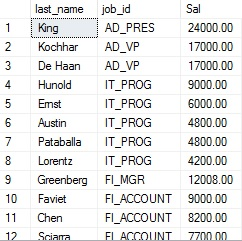
\includegraphics[width=5cm]{./Imagenes/actividad0101} 
	\end{center}

	\item SELECT * FROM job\_grades;
	\\Es incorrecta, la sentencia correcta sería:
	\\SELECT * FROM jobs;
	\begin{center}
	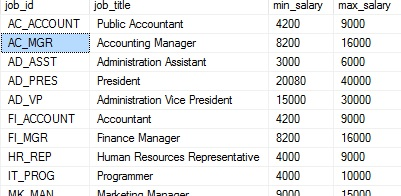
\includegraphics[width=5cm]{./Imagenes/actividad0102} 
	\end{center}
	
	\item SELECT employee\_id, last\_name sal x 12 ANNUAL SALARY FROM employees;
	\\Es incorrecta, la sentencia correcta sería:
	\\SELECT employee\_id, last\_name, salary * 12 'ANNUAL SALARY' FROM employees;
	\begin{center}
	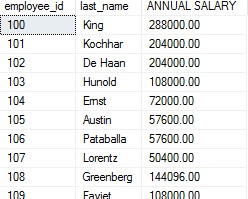
\includegraphics[width=5cm]{./Imagenes/actividad0103} 
	\end{center}

\end{itemize} 